\chapter{جزئیات فنی پروژه}


\section{مقدمه}
در این پروژه از جهت آنکه نسخه قبلی و پیشینی برای  آن نبوده است، به ناچار می‌بایست که کد آن از صفر تا صد آن به صورت دستی نوشته شود. از این‌رو، پیچیدگی های بسیار فراوان را به طور خاص در پی داشت. ابزار های زیادی نیز بنابه شرایط در آن استفاده شد که ارتباط بین آن ابزار ها و اجزا، بر این پیچیدگی پیاده سازی طرح افزوده بود.

ابزار های اصلی و کلی که در این پروژه استفاده شده بود، عبارتند از:

\begin{itemize}
	\item 
	\textbf{نرم افزار پری اسکن}
	\LTRfootnote{PreScan}
	، نسخه \lr{$8.5.0$}
	
	\item 
	\textbf{نرم افزار قدرتمند متلب}
	\LTRfootnote{Matlab}
	، نسخه \lr{R2017b}
	\item 
	\textbf{زبان برنامه نویسی پایتون}
	، نسخه \lr{$3.6.9$}
\end{itemize}

بنابراین برای راه اندازی مجدد کد این پروژه لازم است که موارد بالا روی کامپیوتر شخص به صورت کامل نصب باشد.

همچنین لازم به ذکر است که برخی ابزارات دیگر نیز در این پروژه استفاده شده است که احتمالا با نصب موارد بالا دیگر نیازی به نصب آن ها به صورت جداگانه نیست. هدف این ابزار ها ایجاد اتصال بین اجزای اصلی گفته شده است. این گروه شامل موارد زیر هستند:

\begin{itemize}
	\item 
	\textbf{سیمولینک}
	\LTRfootnote{Simulink}
	، جهت اتصال بین متلب و پری اسکن
	
	\item 
	\textbf{شبکه \lr{UDP}}
	\RTLfootnote{برای این منظور از ماژول \lr{socket} در پایتون استفاده شده است. }
	، جهت اتصال داده های پویا 
	\LTRfootnote{Dynamic Data}
	بین پایتون و سیمولینک
	
	\item 
	\textbf{موتور متلب}
	\LTRfootnote{\matlabengine}
	، جهت اتصال داده های ساکن
	\LTRfootnote{Static Data}
	بین پایتون و سیمولینک
\end{itemize}

در این فصل جزئیات بیشتری در مورد لزوم و دلیل استفاده از این ابزار ها بررسی می‌شود.


\section{دورنمای کلی طرح}
همان‌طور که گفته شد، در این پروژه از ابزار های مختلفی استفاده شده است. برخی ابزارات دیگر نیز جهت ایجاد اتصال بین آن ابزار ها استفاده شده اند. در این بخش، این اجزا به تفصیل بررسی خواهد شد.
 
 هر کدام از این اجزا کار مشخصی را بر عهده دارند.
 شکل  
\ref{fig:block-diagram}
این ارتباط را نشان می‌دهد.

\begin{figure}[h!]
	\centering
	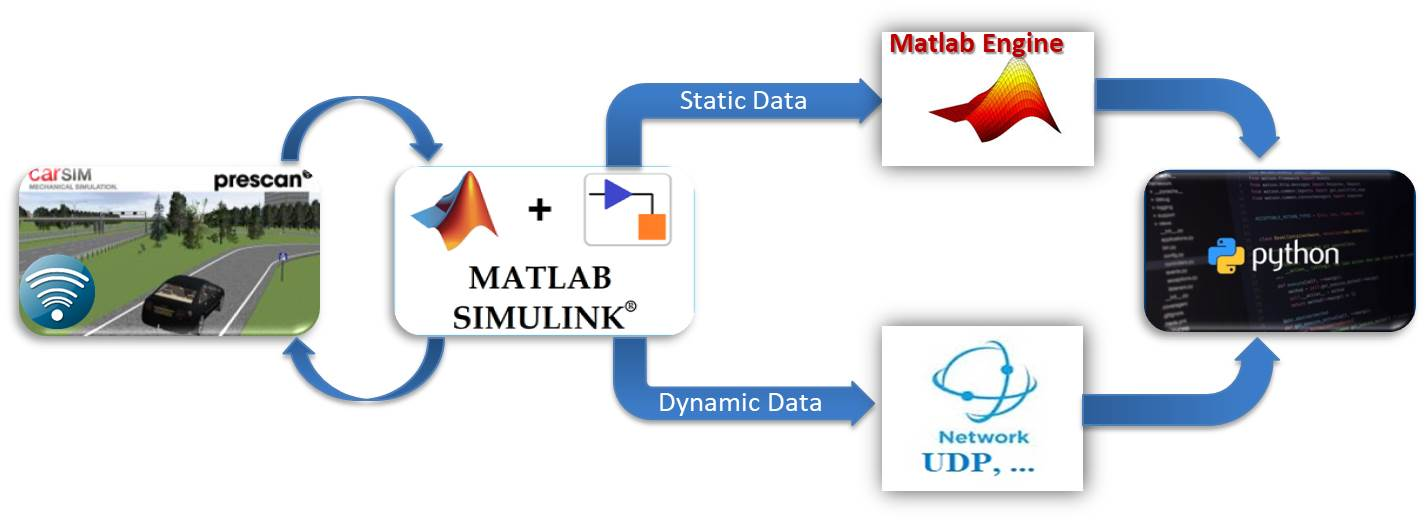
\includegraphics[width=1\linewidth]{Figures/block-diagram-white}
	\caption{بلوک دیالگرام لایه های کلی}
	\label{fig:block-diagram}
\end{figure}

در شکل 
\ref{fig:block-diagram}
از سمت چپ به راست اجزا یاد شده و نحوه ارتباط آن‌ها با‌یک‌دیگر را به‌خوبی نشان می‌دهد. این بلاک ها و ارتباط ها عبارتند از:

\begin{itemize}
	\item 
	اولین بلاک آن، نرم افزار \textbf{پری‌اسکن }می‌باشد. وظیفه اصلی این نرم افزار، شبیه سازی دینامیک یک اتومبیل و یا موتور و ... می‌باشد. همچنین ایجاد یک محیط گرافیکی زیبا و یک پنل کاربری گرافیکی برای ساخت ماشین ها از دیگر حسن های این نرم افزار است.
	
	فایل های مهم ایجاد شده توسط این بخش، \texttt{.pex} و \texttt{.pb} می‌باشد.
	
	\item
	بلاک بعدی ترکیبی از \textbf{متلب و سیمولینک }است. چرا که نرم افزار پری‌اسکن این امکان را دارد که برای کنترل و دسترسی بیشتر به قسمت های کنترلی مختلف، چیزی به نام \lr{API} ارائه می‌دهد. این \lr{API} یک فایل سیمولینک را در اختیار کابران قرار میدهد که در آن بلوک های مشخصی به یکدیگر متصل هستند و با مطالعه و تغییر آن بلوک ها می‌توان کنترل سیستم را به دست گرفت.
	
	فایل های مهم این بخش نیز در فرمت \texttt{.slx} و \texttt{.m} در دسترس هستند.
	
	همچنین \api یاد شده، دستورات دیگری را جهت دریافت داده های استاتیک محیط ساخته شده در این نرم افزار را به کاربران خویش در محیط متلب می‌دهد.

	\item
	دو بلوک بعدی، مربوط به اتصال بین متلب و یا سیمولینک با پایتون هستند. 
	
	بلوک بالایی این اتصال را بین داده های استاتیک شامل طول جاده و عرض هر لاین، موقعیت اولیه اتومبیل و جاده، و بسیاری اطلاعات دیگر که بسیاری از آن اطلاعات استفاده نشده اند زیرا در این پروژه مفید نبوده اند. این بلوک، فایل سیمولینک را تغییر نمی‌دهد.
	
	بلوک پایینی نیز با استفاده از روش های شبکه کردن، می‌تواند داده های پویا را از محیط سیمولینک به پایتون منتقل کند. این داده های پویا عبارتند از موقعیت و سرعت و اطلاعات دیگری از اتومبیل در حال حرکت، اطلاعات سنسورها و ... باشد.
	
	\item 
	بلوک بعدی پایتون است که خود شامل لایه های دیگری است که در شکل 
	\ref{fig:python-layers}
	به تفضیل بیان شده است. نکته جالب در آن این است که در آن لایه ها اثری نیز از دو بلوک پیشین آمده است. همچنین بخش اصلی کار، یا به عبارتی مغز و هوش این کار در این قسمت توسعه یافته است.
\end{itemize}
\subsection{تقسیم بندی وظایف هر بخش}
بخش اصلی کار که وظیفه آن تصمیم گیری و انتخاب مسیر درست توسط یک عامل
\LTRfootnote{Agent}
(که در این پروژه، عامل همان اتومبیل می‌باشد) در پایتون انجام می‌شود. وظیفه اصلی بخش متلب و سیمولینک و پری‌اسکن، ایجاد یک محیط شبیه سازی است. 

\begin{note}


این محیط شبیه سازی اهمیت زیادی در الگوریتم های یادگیری تقویتی دارد. زیرا در این الگوریتم ها یک «عامل» با «محیط
\LTRfootnote{Environment}
» در تعامل است. تعامل در این الگوریتم ها به معنای این است که «عامل» در یک «حالت
\LTRfootnote{State}
» قرار دارد. سپس متناسب با آن یک «حرکت
\LTRfootnote{Action}
» انجام می‌دهد. با این «حرکت»، «محیط» به آن یک مقدار «امتیاز» و یک «حالت» جدید بر‌می‌گرداند. 
بنابراین داشتن یک محیط شبیه سازی کامل و دقیق از اجزای ضروری کار است.

\end{note}

بخش های دیگر مربوط به ارتباط این قسمت ها به یک‌دیگر بودند که پیچیدگی های زیادی را رقم زده است.

به طور ساده‌تر و کلی‌تر می‌توان گفت که پایتون نقش «عامل» و پری‌اسکن نقش «محیط» را دارد.

\section{معرفی نرم افزار پری‌اسکن}
می‌توان در ابتدا گفت که این نرم‌افزار یک افزونه متلب و سیمولینک است اما توانایی زیادی که آن دارد باعث می‌شود که بگوییم این محصول از متلب و سیمولینک جعت رسیدن به هدف خود کمک می‌گیرد.

نرم افزار پری‌اسکن یکی از نرم افزار های بسیار قدرتمند در زمینه شبیه سازی مسایل مربوط به وسایل نقلیه است که می‌تواند حرکت یک ویله نقلیه را به طور خیلی دقیق و مناسب شبیه سازی کند. همچنین در کنار این وظیفه مهم، یک محیط گرافیکی مناسب را در اختیار کاربران خود قرار می‌دهد که از دیگر حسن های آن است.
شکل 
\ref*{fig:prescan-gallery} این توانایی ها را به تصویر کشیده است.
 
همچنین این نرم افزار یک سری فایل خروجی به کاربر می‌دهد که یکی از فایل های آن فایل سیمولینک است که اجازه تغییر و دسترسی به داخل برخی بلاک ها به ما کمک می‌کند که اطلاعات خود را از دل آن نرم افزار بیرون بکشیم.
\RTLfootnote{جهت کسب اطلاعات بیشتر و تهیه این نرم افزار به لینک زیر مراجعه کنید:
\\
\lr{\href{https://tass.plm.automation.siemens.com/prescan}{https://tass.plm.automation.siemens.com/prescan}}
}

از این رو در مقابسه با محیط های دیگر، محاسن زیادی را داشت که هدف این پروژه را در به کار‌گیری این ابزار تحت تاثیر قرار داد.



\begin{figure}
	\centering
	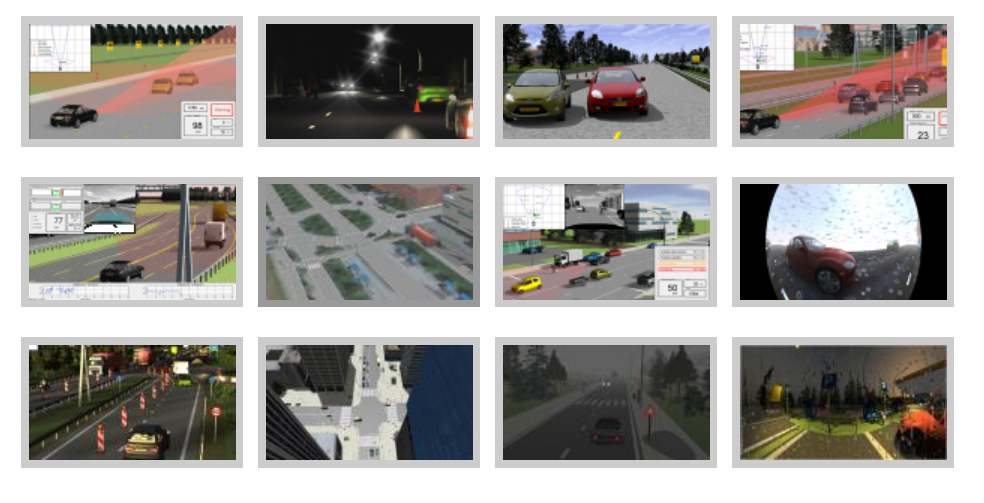
\includegraphics[width=0.8\linewidth]{Figures/Prescan-gallery}
	\caption{بخشی از توانایی های نرم افزار پری‌اسکن در شبیه سازی}
	\label{fig:prescan-gallery}
\end{figure}





\subsection{بخش های مختلف نرم افزار پری‌اسکن}
پس از دانلود و نصب نسخه \lr{8.5.0} این نرم‌افزار چهار آیکون مانند شکل 
\ref{fig:prescan-icons}
به محیط دسکتاپ اضافه می‌کند.  اصلی ترین آن ها 
\lr{PreScan Proccess Manager 8.5.0}
نام دارد.

\begin{figure}[h]
	\centering
	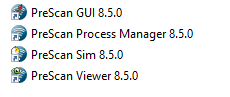
\includegraphics[width=0.4\linewidth]{Figures/prescan-icons}
	\caption{آیکون های اضافه شده بر روی محیط دسکتاپ پس از نصب پری‌اسکن}
	\label{fig:prescan-icons}
\end{figure}
 
 با انتخاب آن صفحه ای مانند زیر باز می‌شود.

\begin{figure}[h]
	\centering
	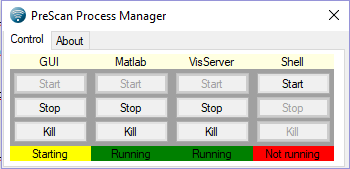
\includegraphics[width=0.5\linewidth]{Figures/Prescan-panel}
	\caption{پنل مدریت نرم‌افزار پری‌اسکن}
	\label{fig:prescan-panel}
\end{figure}

این پنجره شامل گزینه های زیر است:
\begin{multicols}{2}
\begin{itemize}
	\item \lr{GUI}
	\item \lr{VisServer}
	\item \lr{Matlab}
	\item \lr{Shell}
\end{itemize}
\end{multicols}

برای ایجاد یک محیط جدید باید \lr{GUI} را استارت کرد. پس از مدتی صفحه ای مانند شکل 
\ref{fig:prescan-gui}
باز می‌شود. 





\begin{figure}
	\centering
	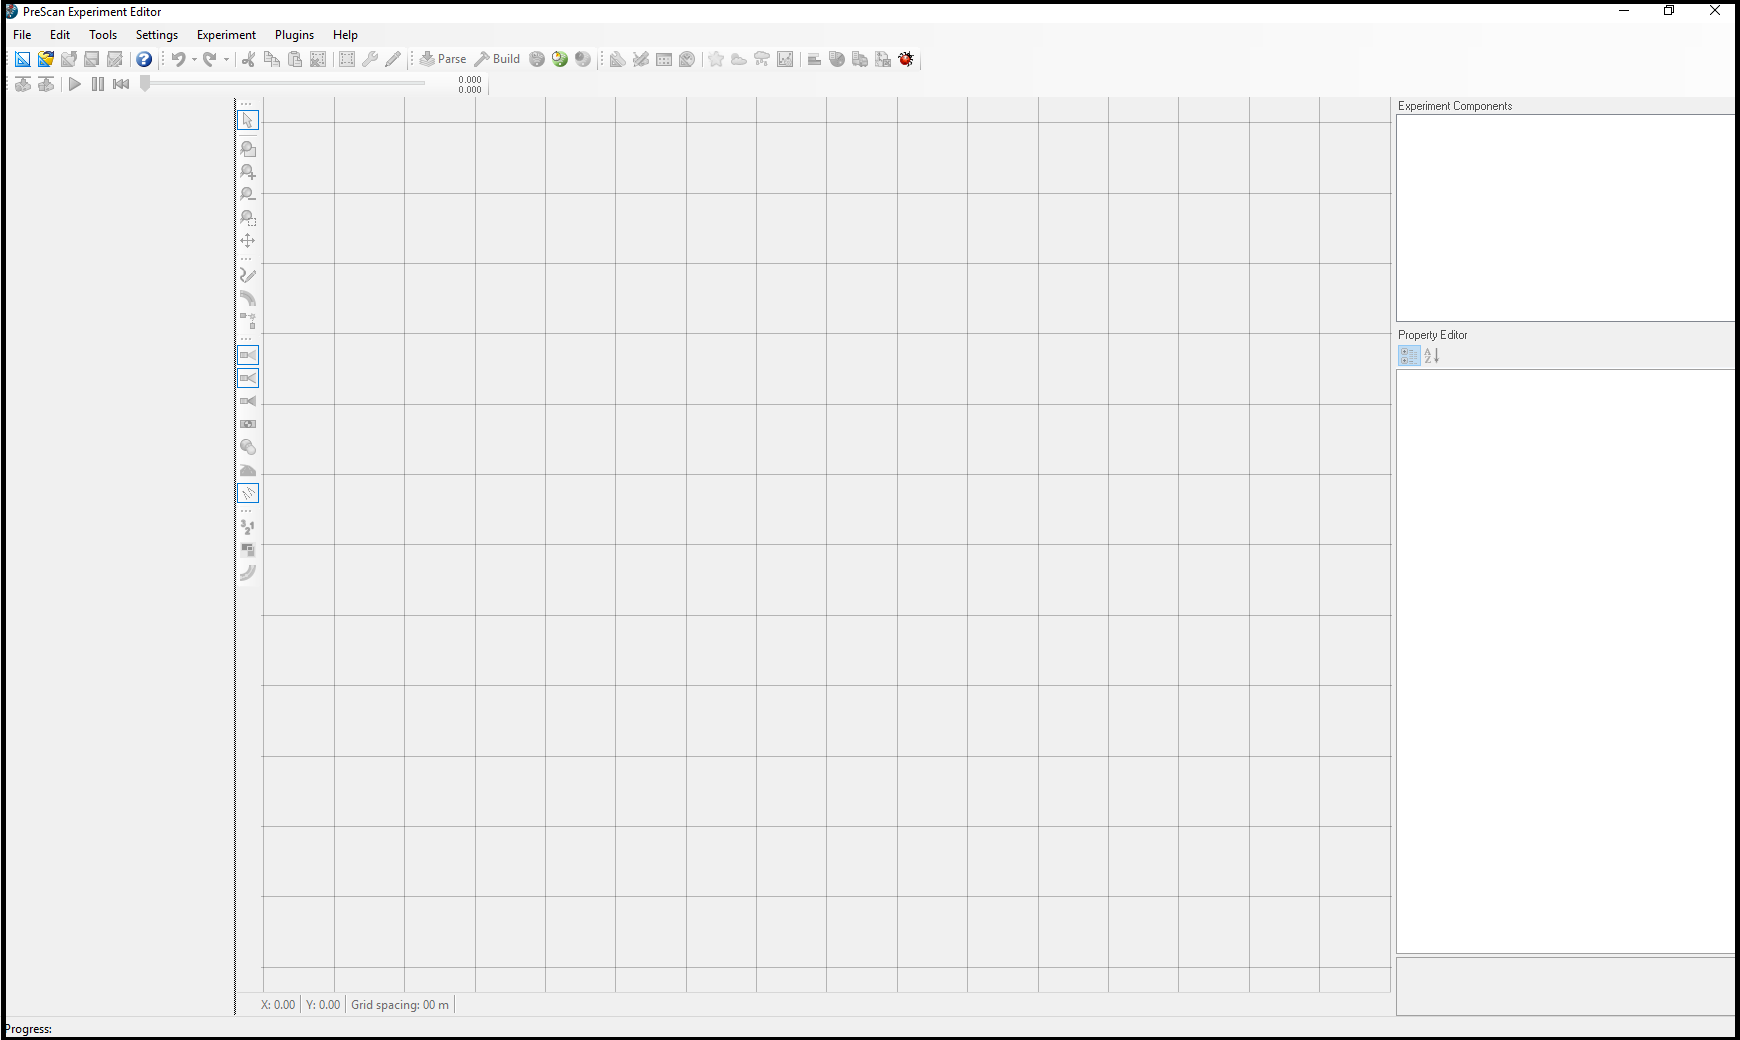
\includegraphics[width=0.7\linewidth]{Figures/Prescan-GUI}
	\caption{صفحه گرافیکی محیط پری‌اسکن}
	\label{fig:prescan-gui}
\end{figure}



پس از ایجاد مدل ها و ذخیره آن، فایل های \texttt{**.pex} و \texttt{**.pb} و \texttt{**\_cs.slx} ساخته می‌شود.
\RTLfootnote{علامت ** به معنای یک اسم مشترک در این سه فایل استفاده شده است. }

جهت استفاده از فایل سیمولینک باید در شکل 
\ref{fig:prescan-panel}
متلب را استارت کنید.
\begin{remark}
	برای اجرای فایل های سیمولینک خروجی، لازم است که متلب را فقط و فقط با استفاده از نرم افزار پری‌اسکن و با استفاده از پنل مدیریت نرم افزار معرفی شده در شکل 
	\ref{fig:prescan-panel}
	باز شود. در صورتی که به صورت مستقیم این کار انجام شود، به مشکل منتهی می‌شود.
\end{remark}


دو قسمت دیگر نیز در شکل 
\ref{fig:prescan-panel}
وجود دارد که نیازی به استارت کردن آن ها نیست و خودشان در صورت لزوم به صورت خودکار فراخوانی می‌شوند.


\subsection{فرمت های فایل های خروجی}
نرم‌افزار پری‌اسکن پس از ایجاد یک محیط جدید، فایل ها و پوشه های بسیار زیادی را ایجاد می‌کند. اما در خارج آن پوشه ها ۳ فایل وجود دارد که پسوند آن ها \texttt{**.pex} و \texttt{**.pb} و \texttt{**\_cs.slx} می‌باشد. علامت ** همان اسم پروژه‌ای است که ایجاد کرده ایم. هر یک از این فایل ها به یک بلوک از شکل 
\ref{fig:block-diagram}
مربوط می‌شود.

\begin{table}[h!]
\tableset{
%{\setcellgapes{0.5em}\makegapedcells
\begin{tabular}{|C{0.15\linewidth}|p{0.8\linewidth}|}
	\hline\rowcolor{lightgray}
	فرمت فایل
	&
	توضیحات 
	\\\hline\hline
	\texttt{**.pex} &	این فایل مربوط به اولین بلوک شکل
	\ref{fig:block-diagram}
	است و ارتباط مستقیم با \lr{GUI} دارد. برای تغییر محیط گرافیکی باید این فایل را باز کرد.
	\\ \hline   
	\texttt{**.pb} & این فایل برخی از اطلاعات فایل 
	\texttt{**.pex}
	را در اختیار دارد و با تغییر آن فایل این فایل نیز عوض می‌شود. این فایل حاوی اطلاعات استاتیک محیط ایجاد شده است و مهم ترین کاربرد آن در بلوک موتور متلب که در شکل 
	\ref{fig:block-diagram}
	نشان داده شده است می‌باشد. پایتون از طریق این فایل این اطلاعات را دریافت می‌کند.
	\\\hline
	\texttt{**\_cs.slx} &
	این فایل سیمولینک است که برای کار کردن با آن باید از پنل مدیریت شکل
	\ref{fig:prescan-panel}
	استفاده کرد. این فایل پس از ایجاد از فایل 
	\texttt{**.pex}
	مستقل می‌شود. این فایل خود قابلیت تغییر دارد و می‌توان بلوک‌های آن‌را در محیط سیمولینک تغییر داد و بلوک های دیگری به آن افزود.  در صورتی که فایل \texttt{**.pex} تغییر کند، این امکان را نیز دارد که از داخل خود سیمولینک با فشردن دکمه ای این تغییرات جدید اعمال شود بدون آن که به تغییرات خود کاربر لطمه ای وارد شود. در این پروژه این فایل، تغییرات بسیاری را تجربه کرد.
	\\\hline
\end{tabular}}
\caption{توضیحات فرمت فایل خروجی}
\label{tab:prescan-format}
\end{table}



جدول
\ref{tab:prescan-format}
توضیحات لازم را جهت آشنایی با این خروجی ها آورده است.

همچنین در بخش  
\ref{ch:fani|sec:simulink}
در مورد فایل \texttt{**\_cs.slx} توضیحات دقیق‌تری در مورد جزییات آن گفته خواهد شد.

\section{بررسی دقیق‌تر فایل سیمولینک}\label{ch:fani|sec:simulink}

فایل سیمولینک ایجاد شده توسط نرم افزار پری‌اسکن، قابلیت تغییر به دست کاربر را دارد. شکل 
\ref{fig:simulink-firstview}
فایل تغییر‌یافته مربوط به این پروژه را نشان می‌دهد.


\begin{figure}
	\centering
	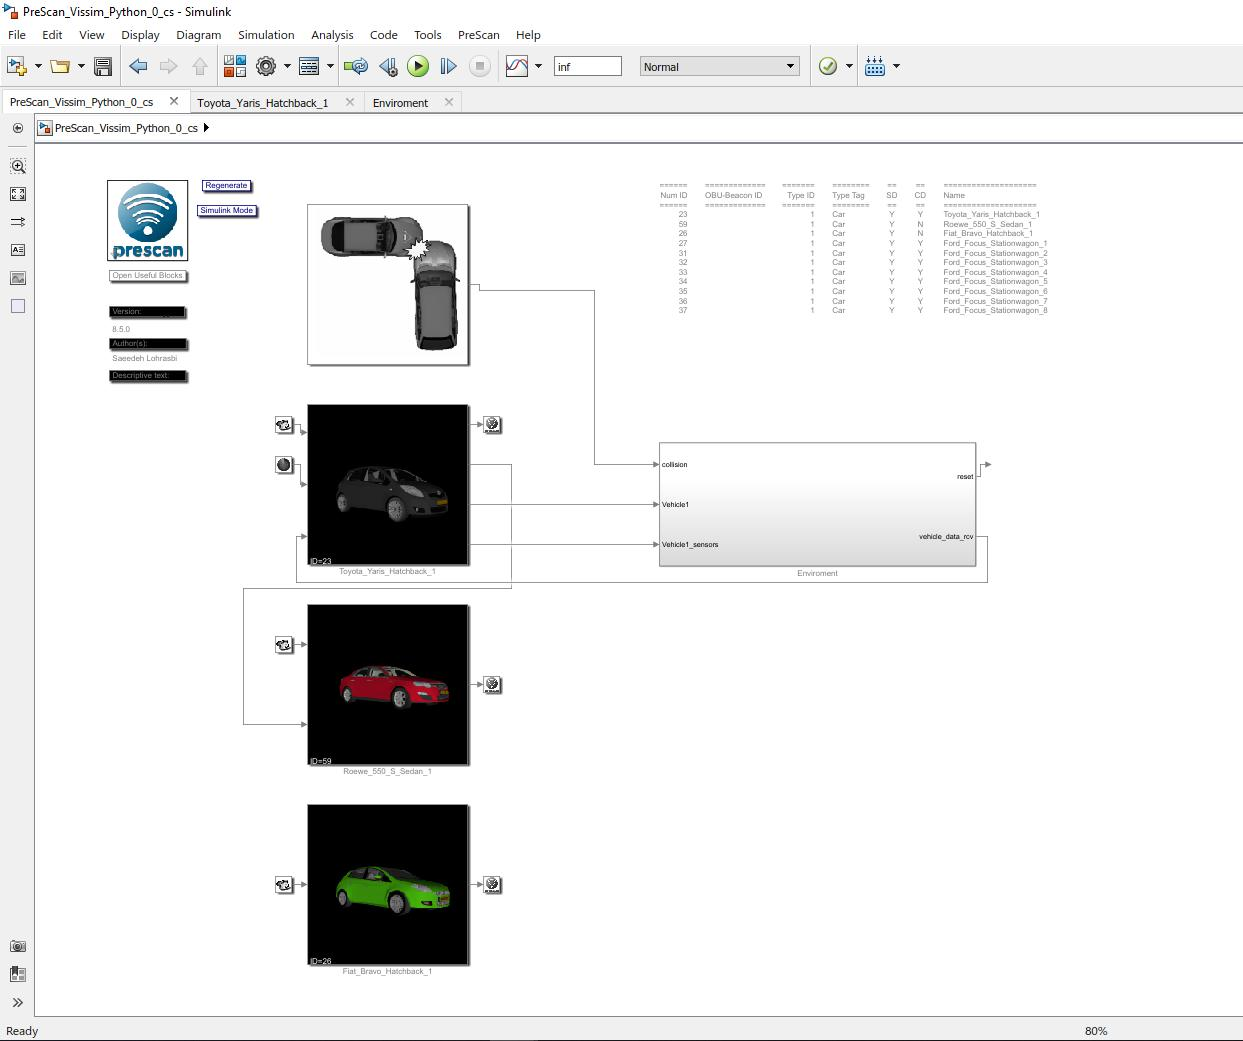
\includegraphics[width=0.7\linewidth]{Figures/simulink/first_view}
	\caption{فایل سیمولینک ایجاد شده توسط نرم افزار پری‌اسکن همراه با تغییرات}
	\label{fig:simulink-firstview}
\end{figure}




بلوک های سمت راست نشان داده شده در سمت راست شکل
\ref{fig:simulink-firstview}
توسط نرم افزار پری اسکن ایجاد شده است که البته دست‌خوش تغییراتی نیز بوده اند. 

در صورتی که با استفاده از محیط گرافیکی \lr{GUI} فایل \texttt{**.pex} تغییر کند، فایل سیمولینک تغییر نمی‌کند. در برخی موارد این تغییرات ممکن است منجر به پیغام خطا شود.

\begin{remark}\label{remark:Regenerate}
	در صورتی که فایل
	 \texttt{**.pex}
	 تغییر کند، برای اعمال این تغییرات، باید روی کلمه 
	 \lr{Regenerate}
	 که در شکل 
	 \ref{fig:simulink-generate}
	 آمده است، کلیک کرد. با این کار، تغییرات جدید اعمال می‌شود بی‌آن‌که تغییرات کاربر تحت تاثیر قرار بگیرد.
\end{remark}

\begin{figure}
	\centering
	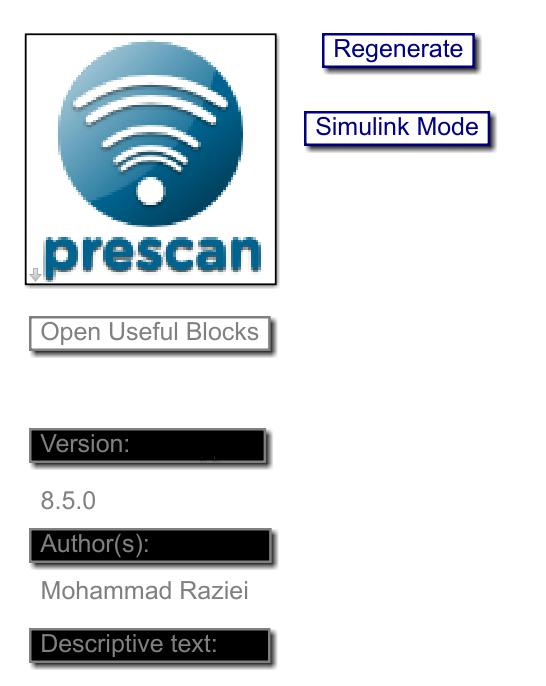
\includegraphics[width=0.4\linewidth]{Figures/simulink/generate}
	\caption{روش صحیح اعمال تغییرات روی فایل سیمولینک}
	\label{fig:simulink-generate}
\end{figure}

در شکل 
\ref{fig:simulink-generate}
همانطور که در نکته
\ref{remark:Regenerate} 
به آن اشاره شد، دکمه ای تحت عنوان 
\lr{Regenerate}
وجود دارد که استفاده از آن در همان نکته مشخص شده است. همچنین در این تصویر در زیر لوگوی برنامه پری‌اسکن، اطلاعاتی مانند شماره نسخه نرم افزار (که در این‌جا \lr{8.5.0} می‌باشد.)، نام نویسنده مشاهده می‌شود.

در شکل 
\ref{fig:simulink-firstview}
اولین بلوک سمت راست همان ماشینی است که ما آن‌را تحت کنترل گرفته‌ایم. اگه به آن وارد شویم، شکل 
\ref{fig:simulink-agent}
را مشاهده می‌کنیم.
در این تصویر ورودی و خروجی ها نقش خیلی مهمی دارند. این اطلاعات در جدول
\ref{tab:simuink-agent-io}
 آمده‌اند.



\begin{figure}[h!]
	\centering
	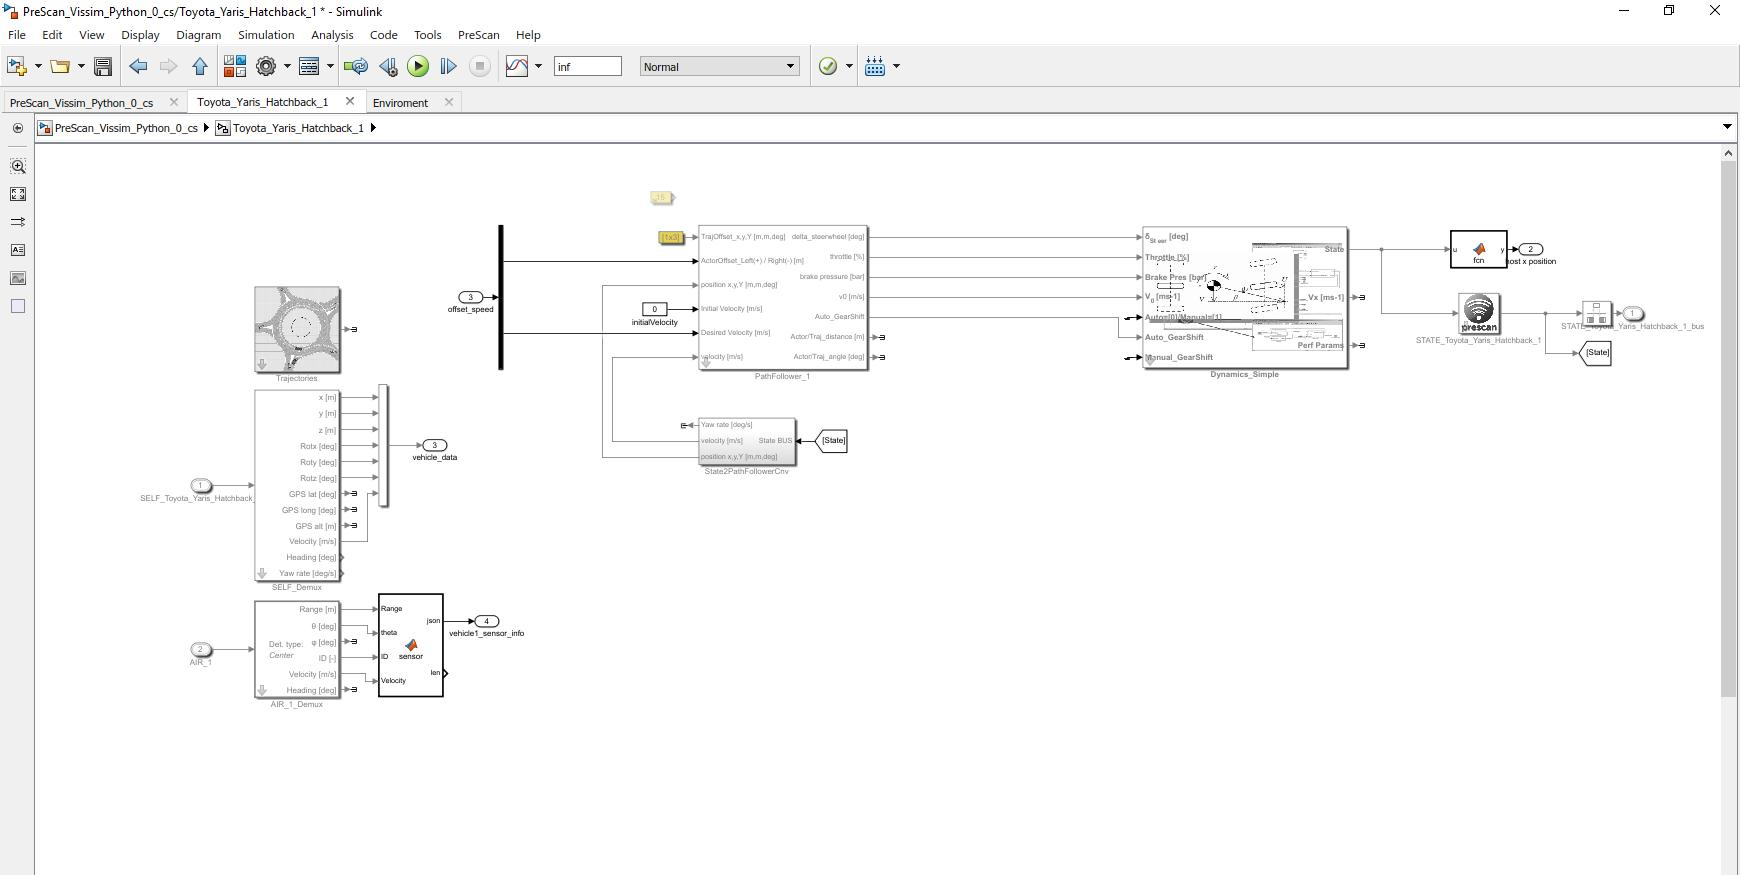
\includegraphics[width=1\linewidth]{Figures/simulink/agent}
	\caption{فایل سیمولینک - شبیه سازی اتومبیل}
	\label{fig:simulink-agent}
\end{figure}


\begin{table}[h!]
	\tableset{
		\begin{tabular}{|C{0.08\linewidth}|C{0.23\linewidth}|C{0.17\linewidth}|p{0.43\linewidth}|}
			\hline\rowcolor{lightgray}
			نوع & عنوان & بلوک مربوط & توضیحات
			\\\hline\hline
			خروجی &اطلاعات ماشین & \lr{SELF\_Demux} & اطلاعات ماشین، شامل اطلاعات موقعیت($x$،$y$ و$z$) و اطلاعات چرخش (حول $x$،$y$ و$z$) به همراه سرعت ماشین را خروجی می‌دهد. این 7 داده قبل از خروجی توسط یک \lr{mux} با یکدیگر ادغام می‌شوند.
			\\\hline
			خروجی& اطلاعات سنسور ماشین & \lr{AIR\_Demux}  & اطلاعات سنسور \lr{V2C} را خروجی می‌دهد. از آنجا که این سنسور فاصله و زاویه و ...  تا ده ماشین نزدیک خود را می‌دهد. بنابراین هر‌یک از این اطلاعات یک بردار ده تایی است. برای فرستادن آن اطلاعات به خروجی، ابتدا آن‌ها را به  طریقی به فرمت جیسون
			\LTRfootnote{json}
			تبدیل می‌کند و یک رشته کاراکتر با طول مشخص
			\RTLfootnote{بعدا خواهید دید که مشخص بودن طول بسیار بسیار اهمیت دارد!}
			را خروجی می‌دهد.
			\\\hline
			ورودی & کنترل لاین و سرعت ماشین & \lr{PathFollower\_1} & دستورات کنترلی اتومبیل، شامل کدام خط بودن و مقدار سرعت نهایی، به صورت ورودی وارد یک \lr{demux} می‌شود و پس از جدا سازی، به بلوک مربوط متصل می‌شود.
			\\\hline
	\end{tabular}}
	\caption{بررسی ورودی ها و خروجی های مهم در شکل \ref{fig:simulink-agent}}
	\label{tab:simuink-agent-io}
\end{table}

در جدول \ref{tab:simuink-agent-io} صرفا ورودی خروجی های مهم مورد بررسی قرار گرفته است. این ورودی ها و خروجی های مهم به یک بلوک دیگر منتقل می‌شود. بلوک 
\lr{Environment}
همان بلوک است که در شکل
\ref{fig:simulink-firstview}
نیز مشخص است و در شکل 
\ref{fig:simulink-env}
نیز از زاویه نزدیک تر با جزییات بیشتر می‌توان آن‌را مشاهده نمود.
%\code[matlab]{simulink-json-sensor.m}



\begin{figure}
	\centering
	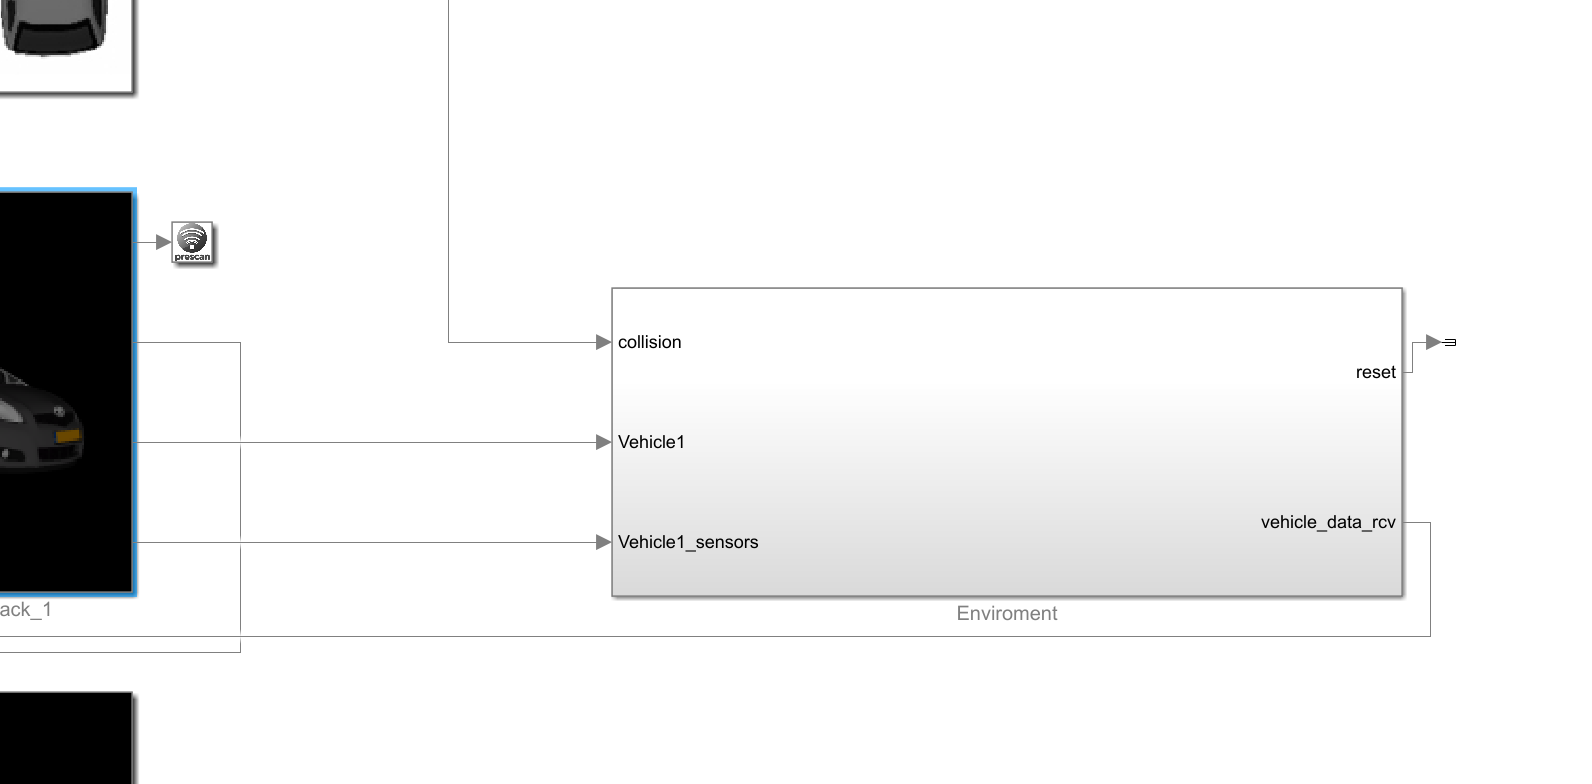
\includegraphics[width=0.7\linewidth]{Figures/simulink/simulink-Env}
	\caption{نگاهی از نزدیک به بلوک \lr{Environmnet}}
	\label{fig:simulink-env}
\end{figure}






%
%
%\begin{figure}[h!]
%	\centering
%	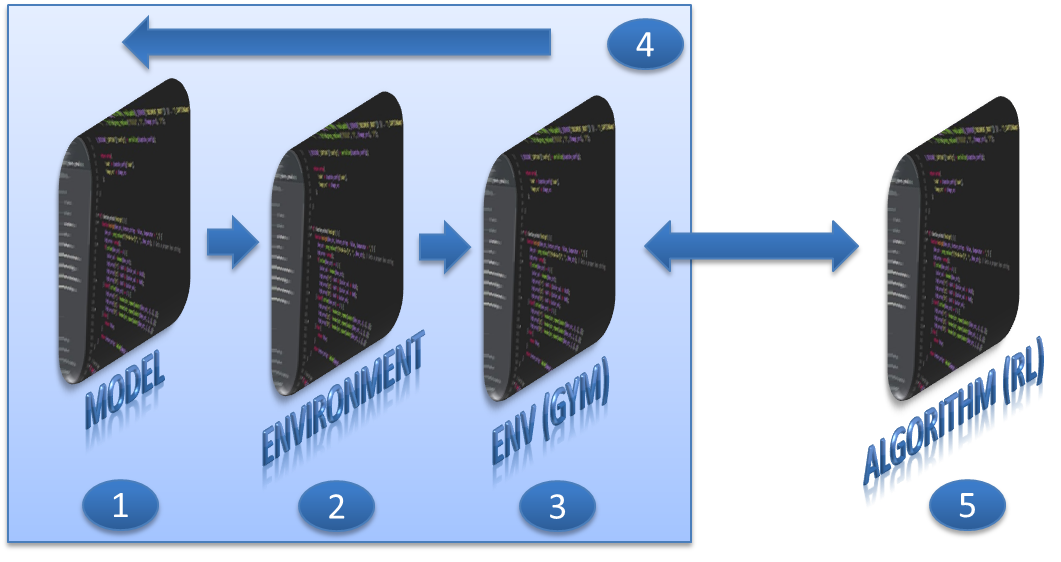
\includegraphics[width=0.7\linewidth]{Figures/python-layers-white}
%	\caption{بلوک دیالگرام لایه های پایتون}
%	\label{fig:python-layers}
%\end{figure}






%\thispagestyle{empty}
%
%\section{مقدمه}
%
%فصل مقدمه یک پایان نامه، با بیان نیاز موضوع، تعريف مسئله و اهمیت آن در یک یا چند بند (پاراگراف) آغاز مي‌شود\footnote{شروع مقدمه نبايد چنان طولاني باشد كه هدف اصلي را تحت‌ تاثير قرار دهد.}  و با مرور پيشينه موضوع (سابقه کارهای انجام‌شده پیشین که ارتباط مستقیمی با مسئله مورد بررسی دارند) ادامه مي‌يابد. سپس در یک یا دو بند توضیح داده مي‌شود كه در این پایان نامه، چه ديدگاه يا راهكار جدیدي نسبت به مسئله (موضوع) مورد بررسي وجود دارد. به‌عبارت دیگر نوآوری‌ها به‌صورت کاملاً شفاف و صریح بیان می‌شود. در ادامه ممکن است به نتايج بدست‌آمده نیز به‌طور مختصر و کلی اشاره ‌شود. در آخرین بند از مقدمه به محتواي فصل‌هاي بعدي پایان نامه به‌اختصار اشاره مي‌شود.\\
%برای مشاهده دستورالعمل کامل دانشگاه صنعتی امیرکبیر(پلی تکنیک تهران) به \cite{zakeri} یا به سایت
%%
%\href{http://library.aut.ac.ir/Thesis%20Guide}{کتابخانه دانشگاه صنعتی امیرکبیر(پلی تکنیک تهران)}%
%مراجعه نمایید.
%
%نگارش صحيح يک پایان نامه در فهم آسان آن بسيار موثر است. در اين فصل مهمترین قواعد نگارشی که باید مورد توجه جدی نگارنده قرار گیرد، به اختصار بیان می‌شود. اين قواعد را مي‌توان در محورهای اصلی زير دسته‌بندی کرد:
%\begin{itemize}
%\item
%فارسی نویسی
%\item
%رعایت املای صحيح 
%\item
%رعایت قواعد نشانه‌گذاری
%\end{itemize}
%\section{فارسی نویسی}
%در حد امکان سعی کنيد به جاي کلمات غير‌فارسی از معادل فارسی آنها استفاده کنيد، به‌ويژه در مواردی که معادل فارسی مصطلح و رايج است‌.‌ به‌طور مثال استفاده از کلمه «لذا» به‌جای «برای همين» يا «به‌همين دليل» توجيهی ندارد‌. همچنين کلمه «پردازش» زيباتر از «پروسس» و معادل فارسی «ريز‌پردازنده» مناسب‌تر از «ميکروپروسسور» است‌.‌ در اين‌گونه موارد چنانچه احتمال عدم آشنايی خواننده با معادل فارسی وجود دارد، يا اصطلاح غير‌فارسی معمول‌تر است، در اولين ظهور کلمه فارسی، اصل غير‌فارسی آن به‌صورت پاورقي آورده شود‌.‌ اگر به‌ناچار بايد کلمات انگليسی در لابه‌لای جملات گنجانده شوند، از هر طرف يک فاصله بين آنها و کلمات فارسی پیش و پس از آنها در‌نظر گرفته شود‌.‌ چنانچه در پایان نامه از مختصر‌نويسی استفاده شود، لازم است در اولين استفاده، تفصيل آن در پاورقي آورده شود‌.‌ 
%
%\section{رعایت املای صحيح }
%رعايت املاي صحيح فارسي به مطالعه و درک راحت‌تر کمک مي‌کند. همچنين در نوشته‌هاي فارسي بايد در حد امکان از همزه « ء، أ، ؤ، ة، إ، ئ» استفاده نشود‌.‌ به‌عنوان مثال «اجزاء هواپیما» و «آئين نگارش» ناصحیح، اما «اجزاي هواپیما» و «آيين نگارش» صحيح هستند.‌
%\section{رعایت قواعد نشانه‌گذاری}
%منظور از نشانه‌گذاري به‌کار‌بردن علامت‌ها و نشانه‌هايي است که خواندن و فهم درست یک جمله را ممکن و آسان مي‌کند. در ادامه نشانه‌هاي معمول و متداول در زبان فارسي و موارد کاربرد آنها به اختصار معرفی می‌شوند.
%
%\subsection{ويرگول}
%ويرگول نشانه ضرورت یک مکث کوتاه است و در موارد زير به‌کار مي‌رود:
%\begin{itemize}
%\item
%در ميان دو کلمه که احتمال داده شود خواننده آنها را با کسره اضافه بخواند، يا نبودن ويرگول موجب بروز اشتباه در خواندن جمله شود.
%\item
%در موردي که کلمه يا عبارتي به‌‌‌‌عنوان توضيح، در ضمن یک جمله آورده شود. مثلاً برای کنترل وضعیت فضاپیماها، به‌دلیل آن‌که در خارج از جو هستند، نمی‌توان از بالک‌های آیرودینامیکی استفاده کرد.
%\item
%جدا‌کردن بخش‌هاي مختلف يک نشاني يا یک مرجع
%\item
%موارد دیگر از این قبیل
%\end{itemize}
%پیش از ويرگول نبايد فاصله گذاشته شود و پس از آن يک فاصله لازم است و بيشتر از آن صحیح نیست.
%\subsection{نقطه}
%نقطه نشانه پایان یک جمله است. پیش از نقطه نبايد فاصله گذاشته شود و پس از آن يک فاصله لازم است و بيشتر از آن صحیح نیست.
%\subsection{دونقطه}
%موارد کاربرد دونقطه عبارتند از:
%\begin{itemize}
%\item
%پيش از نقل قول مستقيم
%\item
%پيش از بيان تفصيل مطلبي که به اجمال به آن اشاره شده‌است.
%\item
%پس از واژه‌اي که معني آن در برابرش آورده و نوشته مي‌شود.
%\item
%پس از کلمات تفسير‌کننده از قبيل «يعني» و ...
%\end{itemize}
%پیش از دونقطه نبايد فاصله گذاشته شود و پس از آن يک فاصله لازم است و بيشتر از آن صحیح نیست.
%\subsection{گیومه}
%موارد کاربرد گیومه عبارتند از:
%\begin{itemize}
%\item
%وقتي که عين گفته يا نوشته کسي را در ضمن نوشته و مطلب خود مي‌آوريم. 
%\item
%در آغاز و پايان کلمات و اصطلاحات علمي و يا هر کلمه و عبارتي که بايد به‌صورت ممتاز از قسمت‌هاي ديگر نشان داده شود.
%\item
%در ذکر عنوان مقاله‌ها، رساله‌ها، اشعار، روزنامه‌ها و ...
%\end{itemize}
%\subsection{نشانه پرسشی}
%پیش از «؟» نبايد فاصله گذاشته شود و پس از آن يک فاصله لازم است و بيشتر از آن صحیح نیست.
%\subsection{خط تیره}
%موارد کاربرد خط تیره عبارتند از:
%\begin{itemize}
%\item
%جدا‌کردن عبارت‌هاي توضيحي، بدل، عطف بيان و ...
%\item
%به‌جاي حرف اضافه «تا» و «به» بين تاريخ‌ها، اعداد و کلمات
%\end{itemize}
%\subsection{پرانتز}
%موارد کاربرد پرانتز عبارتند از:
%\begin{itemize}
%\item
%به‌معني «يا» و «يعني» و وقتي که یک کلمه يا عبارت را براي توضيح بيشتر کلام بياورند.
%\item
%وقتي که نويسنده بخواهد آگاهي‌هاي بيشتر (اطلاعات تکميلي) به خواننده عرضه کند.
%\item
%براي ذکر مرجع در پايان مثال‌ها و شواهد.
%\end{itemize}
%نکته: بین کلمه یا عبارت داخل پرانتز و پرانتز باز و بسته نباید فاصله وجود داشته باشد.
%\section{جدا یا سرهم نوشتن برخی کلمات}
%تقريباً تمامي کلمات مرکب در زبان فارسي بايد از هم جدا نوشته شوند؛ به استثناي صفات فاعلي مانند «عملگر»، «باغبان» و يا «دانشمند» و کلماتي نظير «اينکه»، «آنها». در ادامه به نمونه‌هايي از مواردي که بايد اجزاي يک کلمه جدا، اما بدون فاصله نوشته شوند، اشاره مي‌شود‌:
%\begin{enumerate}
%\item
%در افعال مضارع و ماضی استمراری که با «می» شروع می‌شوند، لازم است که در عين جدا نوشتن، «می» از بخش بعدي فعل جدا نيافتد‌.‌ برای اين منظور بايد از «فاصله متصل» استفاده و «می» در اول فعل با \lr{SS}\LTRfootnote{Shift+Ctrl+@} از آن جدا شود.‌ به‌طور مثال «می‌شود» به‌جاي «می شود». 
%\item
%	«ها»ی جمع بايد از کلمه جمع بسته‌شده جدا نوشته شود؛ مگر در برخی کلمات مانند «آنها». اين امر در مورد کلمات غير‌فارسي که وارد زبان فارسي شده‌اند و با حرف «ها» جمع بسته می‌شوند، مانند «کانال‌ها» يا «فرمول‌ها» مورد تاکيد است.
%\item
%	حروف اضافه مانند «به» وقتي به‌صورت ترکيب ثابت همراه کلمه پس از خود آورده می‌شوند، بهتر است با \lr{SS} از آن جدا شوند‌.‌ مانند «به‌صورت»، «به‌عنوان» و «به‌‌‌لحاظ»‌.‌ لازم به ذکر است هنگامی که حرف اضافه «به» با کلمه پس از خود معناي قيدي داشته باشد، مثل «بشدت» يا «بسادگي»، بهتر است که به‌صورت چسبيده نوشته شود‌.
%\item
%	کلمات فارسی نبايد با قواعد عربی جمع بسته شوند؛ پس «پيشنهادها» صحيح و «پيشنهادات» اشتباه است‌.‌
%\item
%	اسم‌ها و صفت‌هاي دو‌قسمتي مثل «خط‌چين» و «نوشته‌شده» با \lr{SS} از هم جدا می‌شود‌.‌
%\item
%	شناسه‌ها با \lr{SS} از کلمه اصلي جدا می‌شود‌.‌ مثل «شده‌اند»‌ و «شده‌است». 
%\item
%	‌ «است» هنگامی که نقش شناسه را داشته باشد توسط \lr{SS} از قسمت اصلي جدا می‌شود‌.‌ مانند «گفته‌است»‌.
%\item
%	بند پیشین نبايد باعث افراط در استفاده از فاصله متصل شود. مثلاً عبارت «نوشته می‌شود‌« صحيح و عبارت «نوشته‌می‌شود» ناصحیح است. 
%\item
%	فعل‌هاي دو‌کلمه‌اي که معناي اجزاي آنها کاملاً با معناي کل متفاوت است، بهتر است که با \lr{SS} از هم جدا ‌شوند‌.‌
%\item
%	کلمات مرکب مثل کلمه «دوکلمه‌اي» در عبارت «فعل‌هاي دوکلمه‌اي» و «يادداشت‌برداري».
%\item
%	مصدرهاي دو قسمتي با \lr{SS} از هم جدا می‌شوند‌.‌ مثل «ذوب‌کردن» و «واردکردن»‌.
%\item
%	 صفات تفضيلي مثل « آسان‌تر».
%\end{enumerate}
%
